\documentclass{article}

\textwidth=6.5in
\textheight=8.5in
\voffset=-54pt
\oddsidemargin=0in
\evensidemargin=0in
\setlength{\parskip}{8pt}
\setlength{\parindent}{0pt}

\usepackage{amsmath, amssymb}
\usepackage{ifthen}

\usepackage[inline]{enumitem}
\setlist{topsep=0pt, parsep=8pt}

\usepackage[rgb,table]{xcolor}\convertcolorsUfalse
\usepackage{graphicx}

% change hyperref options
\PassOptionsToPackage{hyphens}{url}
\usepackage[bookmarks,colorlinks,linkcolor=black,citecolor=blue,pdfstartview=FitH,urlcolor=blue]{hyperref}
\hypersetup{pdfpagemode=UseNone}
\usepackage{bookmark}

\usepackage{graphicx}
\usepackage{multicol}
\usepackage{framed}
\usepackage{array}

\usepackage{icomma}

\usepackage{pifont}

\usepackage{marginnote}
\usepackage[colorinlistoftodos]{todonotes}
\renewcommand{\marginpar}{\marginnote}

\usepackage{soul}

\usepackage{tikz}
\usetikzlibrary{
  matrix,%
  % enables the snake paths
  decorations.pathmorphing,%
  % enables bigger arrows
  decorations.markings,%
  decorations.pathreplacing,%
  decorations.text,%
  calc,%
  patterns,%
  shapes.geometric,%
  arrows,
  decorations.shapes,
  positioning,
  plotmarks,
  intersections
}
\tikzset{>=latex} % sets default arrow type in tikz
\tikzset{font=\normalsize}
\tikzset{mark size=1.5pt, mark options=thin}
\tikzset{pin distance=4pt,
  every pin edge/.style={<-, thin, shorten <= -2pt}}

\interfootnotelinepenalty=10000
\renewcommand{\thefootnote}{(\arabic{footnote})}

\usepackage{multirow, bigdelim}

% change to \usepackage[sols]{handout} to see solutions
\usepackage[]{handout}

\providecommand{\check}{}
\renewcommand{\check}{\ifmmode{\text{ \ding{51} }}\else{\ding{51} }\fi}

\newcommand\iscurrentenumi[1]{%
  \ifthenelse{\equal{#1}{\theenumi}}{}{#1}}
\setenumerate[1]{ref=\#\arabic*}
\setenumerate[2]{ref=\protect\iscurrentenumi{\theenumi}(\alph*)}
\newcommand\enumiiprefix[2]{%
  \ifthenelse{{\equal{#1}{\theenumi}}\AND{\equal{#2}{(\alph{enumii})}}}{}{}%
  \ifthenelse{{\equal{#1}{\theenumi}}\AND{\NOT{\equal{#2}{(\alph{enumii})}}}}{#2}{}%
  \ifthenelse{\equal{#1}{\theenumi}}{}{#1#2}%
}
\setenumerate[3]{ref=\protect\enumiiprefix{\theenumi}{(\alph{enumii})}\roman*}
% Make an environment that puts items in columns, first going across. 
\usepackage{tabto}
\newenvironment{enumeratecols}[2][]
{\NumTabs{#2}%
  \begin{enumerate*}[%before={\hspace{\dimexpr-\parindent-1pt}\tab},%
    itemjoin={\tab},#1]}%
  {\end{enumerate*}}

\newlength{\tipmargin}
\makeatletter

\newdimen\SOUL@dimen %new
\def\SOUL@ulunderline#1{{%
    \setbox\z@\hbox{#1}%
    % \dimen@=\wd\z@
    \SOUL@dimen=\wd\z@ %new
    \dimen@i=\SOUL@uloverlap
    \advance\SOUL@dimen2\dimen@i %\dimen@ exchanged too
    \rlap{%
      \null
      \kern-\dimen@i
      % \SOUL@ulcolor{\SOUL@ulleaders\hskip\dimen@}%
      \SOUL@ulcolor{\SOUL@ulleaders\hskip\SOUL@dimen}% new
    }%
    \unhcopy\z@
  }}

\renewenvironment{framed}{
  \setlength{\tipmargin}{\textwidth-\linewidth}
  \advance\@totalleftmargin-\tipmargin
  \def\FrameCommand{\hspace{\tipmargin}\fbox}%
  \advance\linewidth\tipmargin
  \MakeFramed {\advance\hsize-\width \FrameRestore}%
}
{\endMakeFramed}

\makeatother

\definecolor{purple}{rgb}{0.5,0,1.0}

\usepackage{fancyhdr}
\lhead{\textcolor{white}{This content is protected and may not be shared, uploaded, or distributed.}}
\rhead{}
\rfoot{\vspace*{\fill}\footnotesize\textcopyright{} \emph{Harvard Math Ma}}
\renewcommand{\headrulewidth}{0pt}
\pagestyle{fancy}
\begin{document}

\htitle{25. More on Exponentials}

\begin{problemonly}
  \begin{framed}

You should be able to:
    \begin{itemize}[topsep=0pt,partopsep=0pt,parsep=8pt,itemsep=0pt]
    \item Fit an exponential function to two data points, a graph, or a verbal description.

    \item Apply the fact that the derivative of an exponential function is proportional to the function.

    \end{itemize}
  \end{framed}
\end{problemonly}

\begin{enumerate}
\item  \emph{Warm up.} Evaluate the following.

  \note{This isn't related to the rest of today's material. I want to point out that you can evaluate these limits by thinking about the graphs of $\left( \dfrac{1}{3} \right)^x$ and $\left( \dfrac{4}{3} \right)^{-x}$, but you can also just think about what happens if you make $x$ really big or really negative.}  

  \probonly{\begin{multicols}{2}}
    \begin{enumerate}
    \item
      \begin{problem}
        $\displaystyle \lim_{x \to \infty} 4 \left( \frac{1}{3} \right)^x$
      \end{problem}

      \begin{solution}
        When $x$ is a very large positive number, $(\frac{1}{3})^x$ is a very small positive
        number, so $\lim\limits_{x \to \infty} 4 \left( \frac{1}{3} \right)^x=0$.
      \end{solution}

    \item
      \begin{problem}
        $\displaystyle \lim_{x \to -\infty} 4 \left( \frac{1}{3} \right)^x$
      \end{problem}

      \begin{solution}
        When $x$ is a very large negative number, $(\frac{1}{3})^x=3^{-x}$ is a very large positive 
        number, so $\lim\limits_{x \to -\infty} 4 \left( \frac{1}{3} \right)^x=\infty$.
      \end{solution}

    \end{enumerate}
  \probonly{\end{multicols}}

  \pspace{\vfill}

  \probonly{\begin{multicols}{2}}
  \begin{enumerate}[start=3]
  \item
    \begin{problem}
      $\displaystyle \lim_{x \to \infty} 5 - \left( \frac{4}{3} \right)^{-x}$ 
    \end{problem}

      \begin{solution}
        When $x$ is a very large positive number, $(\frac{4}{3})^{-x}=(\frac{3}{4})^x$
        is a very small positive
        number, so $\lim\limits _{x \to \infty} 
        \left[5- \left( \frac{4}{3} \right)^{-x}\right]=5$.
      \end{solution}

  \item
    \begin{problem}
      $\displaystyle \lim_{x \to -\infty} 5 - \left( \frac{4}{3} \right)^{-x}$ 
    \end{problem}

    \begin{solution}
        When $x$ is a very large negative number, $(\frac{4}{3})^{-x}$
        is a very large positive
        number, so $\lim\limits _{x \to -\infty} 
        \left[5- \left( \frac{4}{3} \right)^{-x}\right]=-\infty$.
    \end{solution}

  \end{enumerate}
  \probonly{\end{multicols}}

  \pspace{\vfill}

\item 
  A rabbit population is growing exponentially. On June 1, there are 900 rabbits. 14 days later, there are 1200 rabbits. We'd like to write a formula for $R(t)$, the number of rabbits $t$ days after June 1. Here are two approaches.
  \begin{enumerate}
  \item

    \begin{problem}[\nstretch{1.5}]
      \textbf{Approach 1.} From the given data, we can see that the rabbit population gets multiplied by \fitb{0.25in}{$\frac{4}{3}$} every \probonly{$\vphantom{\dfrac{1}{1}}$}\fitb{0.25in}{$14$} days, so $R(t) =
      \fitb{1in}{900\left(\frac{4}{3}\right)^{t/14}}$. 
    \end{problem}

  \end{enumerate}

  \begin{framed}
    \emph{From previous page:} A rabbit population is growing exponentially. On June 1, there are 900 rabbits. 14 days later, there are 1200 rabbits. We'd like to write a formula for $R(t)$, the number of rabbits $t$ days after June 1.
  \end{framed}

  \begin{enumerate}[resume]
  \item

    \begin{problem}[\vfill]
      \textbf{Approach 2.} Since the population is growing exponentially, we can write $R(t) = C \cdot b^t$; we need to find $C$ and $b$.

      What are $R(0)$ and $R(14)$? How can you use these two facts to find $C$ and $b$? 
    \end{problem}

    \begin{solution}
      We know that $R(0)=900$. Since $R(t) = C \cdot b^t$, 
      we have the equation
      \begin{align*}
       C \cdot b^0 &= 900 \\
       C &= 900
      \end{align*}
      We also know that $R(14)=1200$, so
      \begin{align*}
        900 \cdot b^{14} &= 1200 \\
        b^{14} &= \tfrac{4}{3} \\
        b &= \left(\tfrac{4}{3}\right)^{1/14}
      \end{align*}
      Therefore $R(t) = 900 \left(\frac{4}{3}\right)^{t/14}$.
    \end{solution}

  \item

    \begin{problem}[\stretch{0.25}]
      Which approach do you prefer?
    \end{problem}

  \end{enumerate}

\item  \label{fit-exp-to-data-points-1}

  \begin{problem}[\stretch{1.5}]
    Find an exponential function through the points $(4, 10)$ and $(6, 15)$. (Whenever possible, it's helpful to identify what one output is multiplied by to get the other output.)
  \end{problem}

  \begin{solution}
    An exponential function is of the form $f(x) = ab^x$. We know two points on the graph of $f(x)$. $$10=f(4) =ab^4$$ and $$15=f(6)=ab^6$$ Note that we have two equations and two unknowns. We can divide one equation by another to get an equation about just $b$:
    $$ \frac{15}{10} = \frac{ab^6}{ab^4}=b^2$$
    This means $b =\pm \sqrt{\frac{15}{3}}=\pm \sqrt{\frac{3}{2}}$. 
    The base of an exponential function has to be non-negative so $b= \sqrt{\frac{3}{2}}$. Now we can find $a$:
    \begin{align*} 
    10&=a\bigg(\sqrt{\frac{3}{2}}\bigg)^4 \\
    &= a \left(\frac{9}{4}\right) \\
    a &= \frac{40}{9}
    \end{align*}
    So our exponential function is $f(x) = \frac{40}{9}\cdot
    \left(\frac{3}{2}\right)^{x/2}$.
  \end{solution}

  \probonly{\check \emph{How can you check your answer?}}
\end{enumerate}
\pspace{\newpage}

\note{This is a reminder that both linear functions and exponential functions have ``special'' derivatives: the derivative of a linear function is constant, while the derivative of an exponential function is proportional to the function itself.}

\begin{framed}
  \begin{itemize}
  \item The derivative of a linear function $f(x)$ is \ldots\solonly{\textbf{constant}}

  \item The derivative of an exponential function $f(x)$ is\ldots\solonly{\textbf{proportional to $\bm{f(x)}$; in other words, it's $\bm{k f(x)}$ for some constant $\bm{k}$}}

    \probonly{\bigskip}

  \end{itemize}
\end{framed}

\begin{enumerate}[resume]
\item 

  \note{Here we'll apply the idea that $f'(x) = k f(x)$ in a new way.}

  A population of bacteria in a petri dish is growing exponentially. When there are 8000 bacteria, the population is growing at a rate of 400 bacteria per hour.

  \begin{enumerate}
  \item
    \begin{problem}[1.5in]
       How quickly (in bacteria/hr) is the bacteria population growing when there are 10,000 bacteria in the dish?
    \end{problem}

    \begin{solution}
      Let's follow a strategy when dealing with a word problem:
      \begin{enumerate}[label=\arabic*.]
      \item \textbf{Name important things.} This problem is about a population of bacteria over time, so \hl{let $P(t)$ be the population size at time $t$ (where $t$ is measured in hours)}.
      \item \textbf{Figure out the goal.} We are asked, ``How quickly (in bacteria/hr) is the bacteria population growing when there are 10,000 bacteria in the dish?'' This is the same as asking: \hl{When $P(t) = 10,000$, what is $P'(t)$?}
      \item \textbf{Figure out what we know.}
        \begin{itemize}
        \item We are told that $P(t)$ is an exponential function, so we know that \textbf{$\bm{P'(t)}$ is proportional to $\bm{P(t)}$} (that's what {{{{\#7}}(b)}} on \href{https://people.math.harvard.edu/~jjchen/mathma/docs/worksheets/worksheet24-sols.html}{the worksheet ``Derivatives of Exponential Functions''} says); that is, \hl{$P'(t) = k P(t)$ for some constant $k$} (the proportionality constant).
        \item We are also told, ``When there are 8000 bacteria, the population is growing at a rate of 400 bacteria per hour.'' That is, \hl{when $P(t) = 8000$, $P'(t) = 400$}.
        \end{itemize}
      \end{enumerate}
      Now, we'll try to use what we know to get to our goal. We know that $P'(t) = k P(t)$. When $P(t) = 8000$, $P'(t) = 400$, so the equation $P'(t) = k P(t)$ becomes $400 = k \cdot 8000$, and $k = \dfrac{1}{20}$. So, now we know that $P'(t) = k P(t)$ with $k = \dfrac{1}{20}$; in other words, $P'(t) = \dfrac{1}{20} P(t)$. Our goal is to find $P'(t)$ when $P(t) = 10,000$, and we are now perfectly set up to answer that! Since $P'(t) = \dfrac{1}{20} P(t)$, when $P(t) = 10,000$, $P'(t) = \dfrac{1}{20} \cdot 10,000 = \boxed{500}$.
    \end{solution}

  \item

    \begin{problem}[\vfill\newpage]
      If there were 1000 bacteria at time $t=0$ (with $t$ in hours), which of the following is a correct formula for $P(t)$, the number of bacteria at time $t$?

      \begin{enumeratecols}{3}
      \item $P(t) = 1000e^{20t}$
      \item $P(t) = 1000e^{t / 20}$
      \item $P(t) = 50e^t$
      \end{enumeratecols}
    \end{problem}

    \begin{solution}
      We know that $P'(t)=\frac{1}{20}P(t)$. The only choice that matches this
      is choice (ii).
    \end{solution}

  \end{enumerate}

\item   \label{surge-function-1}

  The function $\displaystyle f(x) = \frac{3x}{e^x}$ is an example of a surge function. Surge functions are used to model many situations. For instance, the amount of an IV drug in the blood $x$ minutes after the drug is administered can be modeled as a surge function.

  Our ultimate goal in this problem is to sketch the graph of $f$.

  \begin{enumerate}

  \item

    \note{I will emphasize that $\dfrac{\infty}{\infty}$ limits need more work. Here, we can make an educated guess based on what we know about the graphs of $y = 3x$ and $y = e^x$, but this isn't a general method for approaching $\dfrac{\infty}{\infty}$ limits. (If students are worried about this, reassure them that we don't expect them to be able to deal with $\dfrac{\infty}{\infty}$ limits yet. We'll learn methods in Mb for handling them. They should, however, be comfortable computing $\displaystyle \lim_{x \to -\infty} f(x)$.)
    }

    \begin{problem}[\stretch{0.5}]
      We can evaluate one of $\displaystyle \lim_{x \to \infty} f(x)$ and $\displaystyle \lim_{x \to -\infty} f(x)$. Which one? Do you have a guess as to what the value of the other one is?
    \end{problem}

    \begin{solution}
      We are looking for $\displaystyle \lim_{x \to -\infty} \frac{3x}{e^x}$. As $x \to -\infty$ (in words, as $x$ gets very very negative, or $x$ decreases without bound), $3x \to -\infty$ and $e^x \to 0$. That is, when $x$ is very negative, $3x$ is a very negative number, and $e^x$ is a number very close to 0. When we divide a very negative number by a number very close to 0, we know we get something huge, but we need to figure out whether it's hugely positive or hugely negative. To do this, notice that $e^x$ is always positive, so we're always dividing our very negative number ($3x$) by a tiny \textit{positive} number ($e^x$), which means that our answer will be a huge negative number. In other words, $\displaystyle \lim_{x \to -\infty} f(x) = \boxed{-\infty}$.

      This question is asking for $\displaystyle \lim_{x \to \infty} \frac{3x}{e^x}$. As $x \to \infty$, both the numerator ($3x$) and the denominator ($e^x$) increase without bound. But which increases more quickly? If you think about the graphs of $3x$ and $e^x$ (shown below), you should realize that $e^x$ grows much more quickly than $3x$. Therefore, $\displaystyle \lim_{x \to \infty} \frac{3x}{e^x} = \boxed{0}$.\footnote{If this seems puzzling, here's one way to think about it: looking at the graph as $x$ increases, it's clear that eventually $3x$ is less than half as big as $e^x$, then less than a third as big, then less than a fourth as big, and so on. So, the ratio between the two just gets closer and closer to 0.}
      \begin{center}
        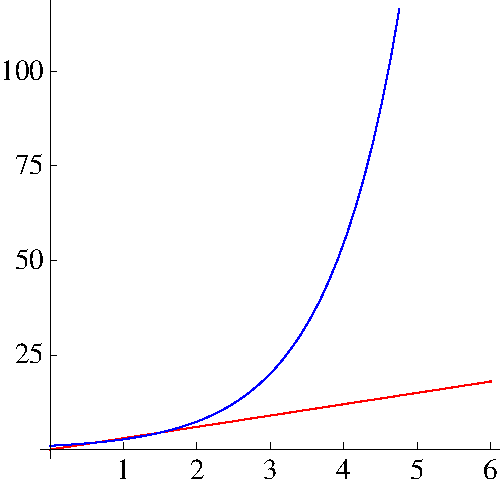
\includegraphics[width=2in]{images/surge-function-1-num-den}
      \end{center}
    \end{solution}

  \item
    \begin{problem}[\vfill]
      Where is $f$ increasing? Where is $f$ decreasing? 
    \end{problem}

    \begin{solution}
         Let's rewrite $f(x)$ as $3xe^{-x}$.  Then, 
        \begin{align*}
          f'(x) &= 3 \frac{d}{dx} \left( x e^{-x} \right) \textrm{ by the
            Constant Multiple Rule} \\
          &= 3 \left[ x \left( \frac{d}{dx} e^{-x} \right) + \left(
              \frac{d}{dx} x \right) e^{-x} \right] \textrm{ by the Product
            Rule} \\
          &= 3 \left( - x e^{-x} + e^{-x} \right) \\
          &= \boxed{\frac{3 (1 - x)}{e^x}}
        \end{align*}
      We already know that $\displaystyle f'(x) = \frac{3 (1 - x)}{e^x}$, so we are simply trying to figure out when this is positive or negative. We first find all the values where the function is either 0 or undefined. In this case, the only such value is $x = 1$. Then, we can break the number line into two intervals, $(-\infty, 1)$ and $(1, \infty)$ and simply test one point in each interval.
      \begin{itemize}
      \item To test the interval $(-\infty, 1)$, we pick a value in the
        interval, like $x = 0$.  When $x = 0$, $\displaystyle \frac{3 (1 -
          x)}{e^x} > 0$, so we know that $f'(x) > 0$ on the entire
        interval $(-\infty, 1)$.
      \item To test the interval $(1, \infty)$, we pick a value in the
        interval, like $x = 2$.  When $x = 2$, $\displaystyle \frac{3 (1 -
          x)}{e^x} < 0$, so we know that $f'(x) < 0$ on the entire
        interval $(1, \infty)$.
      \end{itemize}
      Summarizing, we've found that \fbox{$f$ is increasing on $(-\infty, 1)$ and decreasing on $(1, \infty)$}.
    \end{solution}

  \item
    \begin{problem}[\vfill\newpage]
      Where is $f$ concave up? Where is $f$ concave down? 
    \end{problem}

    \begin{solution}
      The easiest way to answer this is to see when $f''(x)$ is positive and when it is negative. So, our first task is to evaluate $f''(x)$. This means we need to differentiate $\displaystyle f'(x) = \frac{3 (1 - x)}{e^x}$. Let's rewrite it as $f'(x) = 3 (1 - x) e^{-x}$. Then,
      \begin{align*}
        f''(x) &= 3 \frac{d}{dx} \left[ (1 - x) e^{-x} \right] \textrm{ by
          the Constant Multiple Rule} \\
        &= 3 \left[ (1 - x) (-e^{-x}) + (-1) e^{-x} \right] \textrm{ by
          the Product Rule} \\
        &= \frac{3 (x - 2)}{e^x} \textrm{ after a whole bunch of algebra}
      \end{align*}
      To figure out when this is positive or negative, we use the same method as in the previous part: we first figure out when it is 0 (when $x = 2$) or undefined (never). Then, we split the number line at these values, giving us two intervals to check, $(-\infty, 2)$ and $(2, \infty)$.
      \begin{itemize}
      \item To check the interval $(-\infty, 2)$, we pick a value in the interval like $x = 0$. When $x = 0$, $\displaystyle \frac{3 (x - 2)}{e^x} < 0$, so we conclude that $f''(x) < 0$ on $(-\infty, 2)$. Therefore, \fbox{$f$ is concave down on $(-\infty, 2)$}.
      \item To check the interval $(2, \infty)$, we pick a value in the interval like $x = 3$. When $x = 3$, $\displaystyle \frac{3 (x - 2)}{e^x} > 0$, so we conclude that $f''(x) > 0$ on $(2, \infty)$. Therefore, \fbox{$f$ is concave up on $(2, \infty)$}.
      \end{itemize}
    \end{solution}

  \item
    \begin{problem}[1in]
      Find all intercepts of $f$.
    \end{problem}

    \begin{solution}
      Plugging in $x=0$, we find that the $y$-intercept is $\frac{3(0)}{e^0}=\boxed{0}$.
      Solving $\frac{3x}{e^x}=0$ for $x$, we find that the only $x$-intercept is $\boxed{0}$. 
    \end{solution}

  \item
    \begin{problem}[\vfill]
      Use your answers to the previous parts to sketch a graph of $f(x)$. Label asymptotes, intercepts, and the $x$-values of turning points and inflection points. 
    \end{problem}

    \begin{solution}
      We know:
      \begin{itemize}
      \item On $(-\infty, 1)$, $f(x)$ is increasing and concave down (this piece is shown in red below). On $(1, 2)$, $f(x)$ is increasing and concave up (this piece is shown in green below). On $(2, \infty)$, $f(x)$ is decreasing and concave up (this piece is shown in blue).
      \item As $x \to -\infty$, $f(x) \to -\infty$; that is, as we move to the left, the graph decreases without bound.
      \item As $x \to \infty$, $f(x) \to 0$; that is, as $x$ gets bigger, $f(x)$ approaches 0. (So, $y = 0$ is a horizontal asymptote for the graph.)
      \item The peak of the graph is at $\left(1, \frac{3}{e} \right)$.
      \item The $y$-intercept is $0$, and the only $x$-intercept is also $0$.
      \end{itemize}
      So, here is the graph:
      \begin{center}
        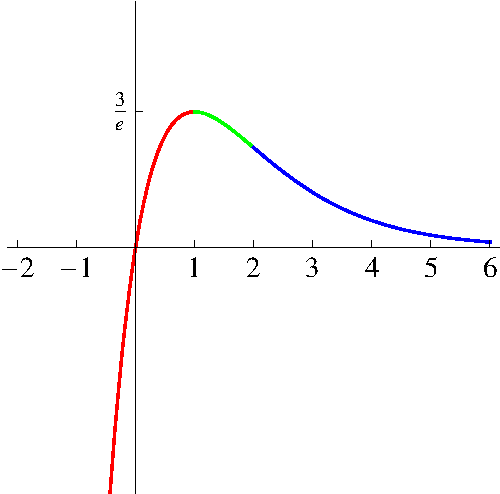
\includegraphics[width=2.5in]{images/surge-function-1}
      \end{center}
    \end{solution}

  \item
    \begin{problem}[\nstretch{0.5}]
      Does $f$ have a global maximum on $(-3, 3)$? If so, where? How about a global minimum?
    \end{problem}

    \begin{solution}
      Looking at our graph, we can determine that the global maximum is achieved
      at $x=1$. There is no global minimum on $(-3, 3)$.
    \end{solution}

  \end{enumerate}

\item 

  \note{It isn't important to do this problem; I put it here just as practice with exponent rules, but I don't really expect to get to it.}

  Suppose $a, b$ are numbers such that $3^a = 10$ and $3^b = \dfrac{1}{7}$. 

  \begin{enumerate}
  \item
    \begin{problem}
      In each statement, fill in the blanks with consecutive integers (for example, 3 and 4).
    \end{problem}

    \begin{itemize}
    \item $a$ is between $\fitb{0.25in}{2}$ and $\fitb{0.25in}{3}$.
    \item $b$ is between $\fitb{0.25in}{-2}$ and $\fitb{0.25in}{-1}$.
    \end{itemize}

    \pspace{\vfill}

  \item
    Simplify the following expressions. (Your answers shouldn't involve $a$, $b$, or $c$.)

    \begin{enumerate}
    \item
      \begin{problem}[\vfill]
        $3^{a + b}$
      \end{problem}

      \begin{solution}
        $3^{a+b} = 3^a 3^b = (10)(\frac{1}{7}) = \frac{10}{7}$.
      \end{solution}

    \item
      \begin{problem}[\vfill]
        $3^{-b}$
      \end{problem}

      \begin{solution}
        $3^{-b} = \frac{1}{3^b} = \frac{1}{1/7} = 7$.
      \end{solution}

    \item
      \begin{problem}[\vfill]
        $3^{2a - b / 4}$
      \end{problem}

      \begin{solution}
        $3^{2a-b/4} = 3^{2a}3^{-b/4} = (3^a)^2(3^b)^{-1/4}=(10)^2(\frac{1}{7})^{-1/4}
        =10^2\cdot 7^{1/4}$.
      \end{solution}

    \item
      \begin{problem}[\vfill]
        $3^{-4a}$
      \end{problem}

      \begin{solution}
        $3^{-4a}=(3^a)^{-4} = 10^{-4}$.
      \end{solution}

    \end{enumerate}

  \end{enumerate}

\end{enumerate}
\end{document}
